\section{Models for signal and background components in invariant mass spectrum}
\label{sec: model}

The expected signal shape, as well as the expected shape for the combinatorial and physical background has to be known in order to properly model the invariant mass distribution of 
$\Bs\to\Ds\kaon\pion\pion$ and $\Bs\to\Ds\pion\pion\pion$ candidates.

\subsection{Signal models for $\m(\Ds\pion\pion\pion)$ and $m(\Ds\kaon\pion\pion)$}
\label{subsec: signalmodel}
The mass distribution of $\Bs\to\Ds\kaon\pion\pion$ signals is modeled using two Gaussian functions, which share the same mean $\mu$, but are allowed to have different widths $\sigma_{1}$ and $\sigma_{2}$. 
Another double Gaussian function is used to account for the contribution of the $\B^{0}\to\Ds\kaon\pion\pion$ decay, which is also present in the $m(\Ds\kaon\pion\pion)$ spectrum. 
All parameters of both double Gaussians, except the core width $\sigma_{1}$, are allowed to float in the fit. 
The core width is fixed to the value obtained from simulation in order to improve the stability of the fit. \newline
The same approach is used to describe the invariant mass distribution of $\Bs\to\Ds\pion\pion\pion$ candidates. 
A double Gaussian function is used to model the signal, all parameters except the core width $\sigma_{1}$ are allowed to float.

\subsection{Background models for $\m(\Ds\pion\pion\pion)$} 
\label{subsec: BkginNorm}
Different background sources arise in the invariant mass spectrum of candidates in the normalization mode. \newline
The following backgrounds have to be accounted for:
\begin{itemize}

\item Combinatorial background: This contribution arises from either a real $\Ds$, which is paired with random tracks to form the $\Bs$ candidates, or via real $X_{d}$'s, which are combined with three tracks that fake a $\Ds$ candidate to form a fake $\Bs$.   

\item Partially reconstructed $\Bs\to\Ds^{*}\pion\pion\pion$ decays, with $\Ds^{*}\to\Ds\gamma$ or $\Ds^{*}\to\Ds\piz$, where the $\gamma$/$\piz$ is not reconstructed in the decay chain. 

\end{itemize}

In both cases of combinatorial background, the distribution in the invariant mass of $\Bs$ candidates is expected to be smooth and decrease with higher masses. 
Therefore, one exponential function is used to model these contributions. \newline
The shape of the  $\Bs\to\Ds^{*}\pion\pion\pion$ contribution is expected to be peaking in the $m(\Ds\pion\pion\pion)$ spectrum, with large tails due to the missing momentum, which is carried away by the $\piz$ or $\gamma$. 
The pion or photon from $\Ds^{*}\to\Ds(\gamma/\piz)$ is excluded from the reconstruction. 
We model the shape of this contribution using the sum of three bifurcated Gaussian functions.
%\begin{figure}[h]
%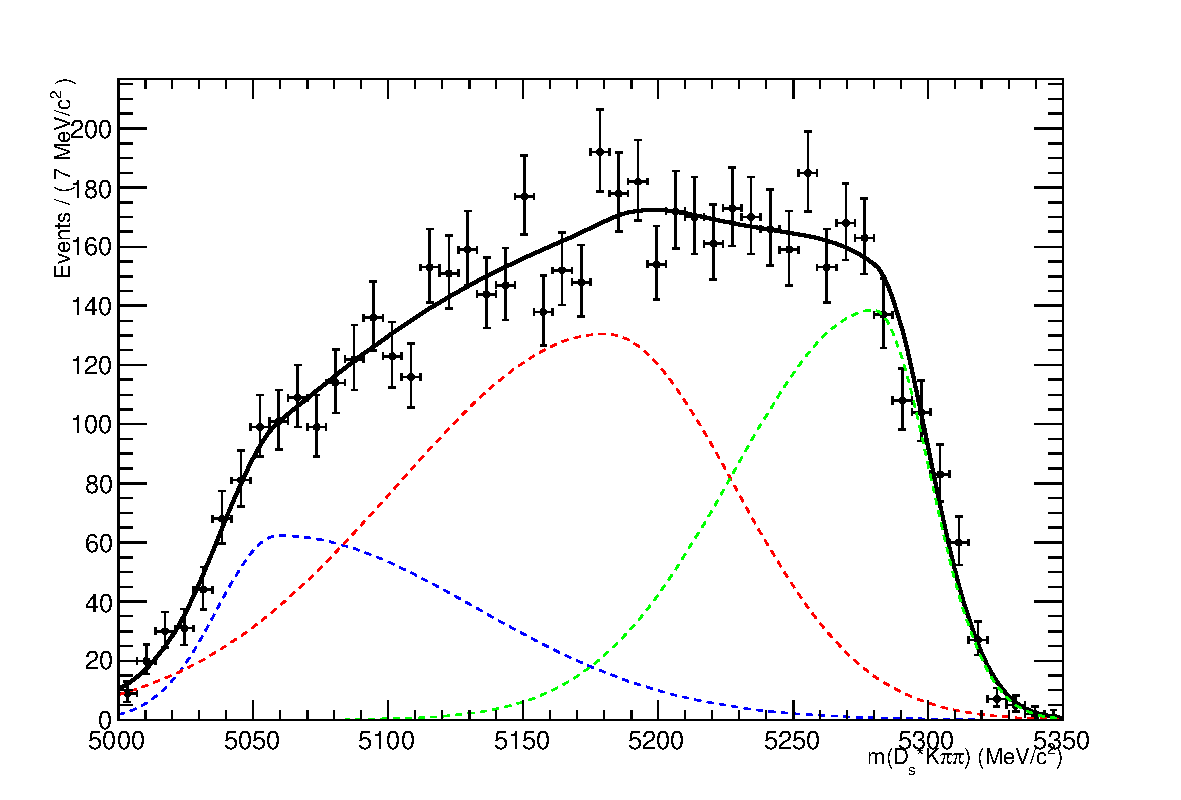
\includegraphics[height=8.cm,width=0.80\textwidth]{figs/Bs2Dsstartpipipi.pdf}
%\caption{Invariant mass distribution of simulated $\Bs\to\Ds^{*}\pion\pion\pion$ events, where the $\gamma$/$\piz$ is excluded from the reconstruction. 
%A fit of the sum of three bifurcated Gaussian functions to this distribution is overlaid.}
%\label{fig: BsDsstar3piMC}
%\end{figure}
%Figure \ref{fig: BsDsstar3piMC} shows the fit of the sum of three bifurcated Gaussian functions to the invariant mass distribution of simulated $\Bs\to\Ds^{*}\pion\pion\pion$ event. 
The shape parameters, 
%are used as input values for the nominal $m(\Ds\pion\pion\pion)$ mass fit. 
as well as the yield of this contribution, are directly determined on data from a fit to the $m(\Ds\pion\pion\pion)$ invariant mass distribution. 

\subsection{Background models for $m(\Ds\kaon\pion\pion)$}
For the signal channel, the following background sources have to be considered:

\begin{itemize}

\item Combinatorial background: same contributions as discussed in Sec. \ref{subsec: BkginNorm}.

\item Partially reconstructed $\Bs\to\Ds^{*}\kaon\pion\pion$ decays, with $\Ds^{*}\to\Ds\gamma$ or $\Ds^{*}\to\Ds\piz$, where the $\gamma$/$\piz$ is not reconstructed in the decay chain. 

\item Partially reconstructed $\Bz\to\Ds^{*}\kaon\pion\pion$ decays, with $\Ds^{*}\to\Ds\gamma$ or $\Ds^{*}\to\Ds\piz$, where the $\gamma$/$\piz$ is not reconstructed in the decay chain.

\item Misidentified $\Bs\to\Ds\pion\pion\pion$ decays, where one of the pions is wrongly identified as a kaon $\pion\rightarrow\kaon$.  

\item Misidentified, partially reconstructed $\Bs\to\Ds^{*}\pion\pion\pion$ decays, where one of the pions is wrongly identified as a kaon $\pion\rightarrow\kaon$ and the $\gamma$/$\piz$ from $\Ds^{*}\to\Ds\gamma$/$\piz$ is 
not reconstructed.

\end{itemize}

The combinatorial background is expected to be non-peaking in the spectrum of the invariant mass of $\Bs\to\Ds\kaon\pion\pion$ candidates. An exponential function is used to model this contribution.\newline
The shape of the partially reconstructed background without misID is taken from our normalization channel, where it can be directly fitted by the sum of three bifurcated Gaussian functions as described above.
In the signal mass fit, all shape parameters for the $\Bs\to\Ds^{*}\kaon\pion\pion$ background are fixed to the input values from our normalization fit.  
%A MC sample of $\Bs\to\Ds^{*}\kaon\pion\pion$ events, where the $\gamma$/$\piz$ is excluded from the reconstruction, is generated. 
%The sum of three bifurcated gaussians is then fitted to the mass distribution of $\Bs$ candidates. The distribution and the overlaid fit is shown in Fig. \ref{fig: BsDsstarKpipiMC}.  

%\begin{figure}[h]
%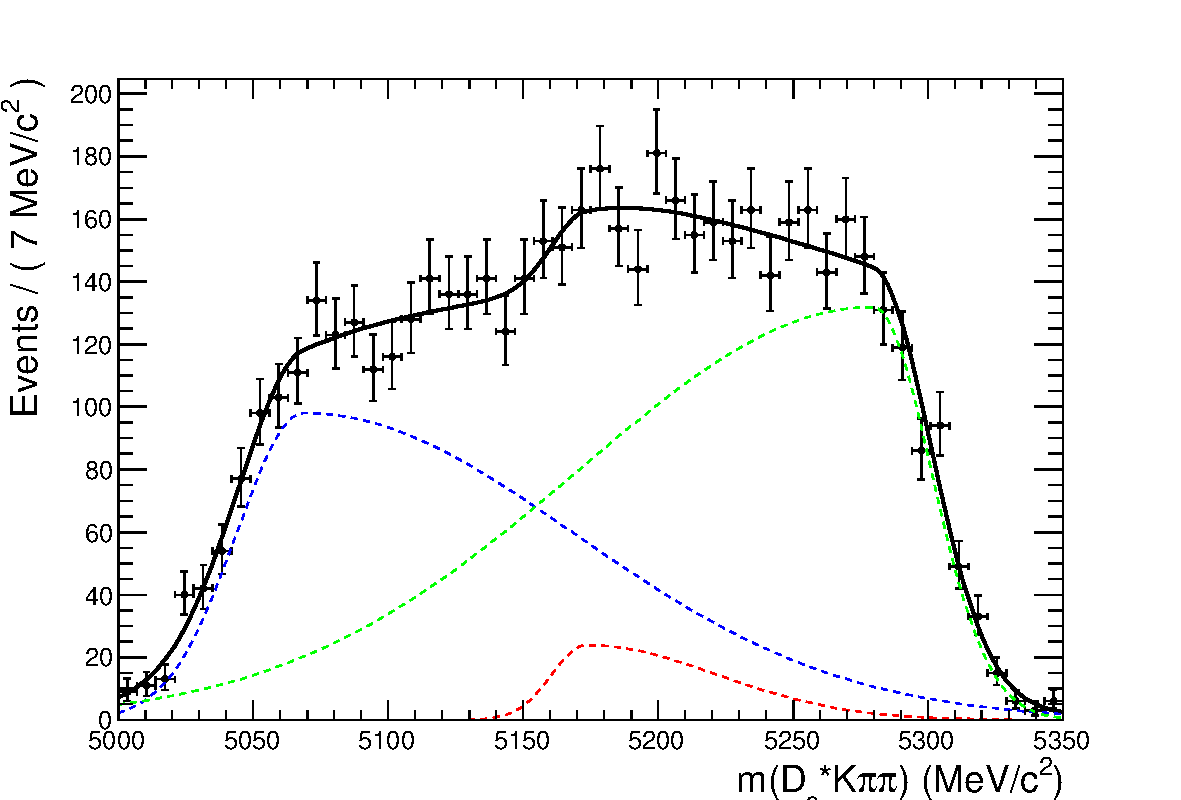
\includegraphics[height=8.cm,width=0.80\textwidth]{figs/Bs2DsstartKpipi.pdf}
%\caption{Invariant mass distribution of simulated $\Bs\to\Ds^{*}\kaon\pion\pion$ events, where the $\gamma$/$\piz$ is excluded from the reconstruction. 
%A fit of the sum of three bifurcated gaussians to this distribution is overlaid.}
%\label{fig: BsDsstarKpipiMC}
%\end{figure}

For the contribution of the $\Bz\to\Ds^{*}\kaon\pion\pion$ background, the same shape is used but the means $\mu_{i}$ of the bifurcated gaussians are shifted down by $m_{\Bs} - m_{\Bz}$ \cite{Agashe:2014kda}. 
The yields of both contributions are directly determined in the nominal fit. \newline
To determine the shape of misidentified $\Bs\to\Ds\pion\pion\pion$ candidates in the $m(\Ds\kaon\pion\pion)$ spectrum, we take a truth-matched signal MC sample of our normalization channel. 
We then use the PIDCalib package to determine the $\pion\rightarrow\kaon$ fake rate. For every candidate in our MC sample, a (momentum) $\ptot$ and (pseudorapidity) $\eta$-dependent event weight is computed and assigned. 
We flip the particle hypothesis from pion to kaon for the $\pion$ with the biggest miss-ID weight for each event and recompute the invariant $\Bs$ mass. This distribution is then modeled using two Crystal Ball functions. 
The distribution and the fit are shown in Fig. \ref{fig: BsDspipipiMCmissID}(left). 

\begin{figure}[h]
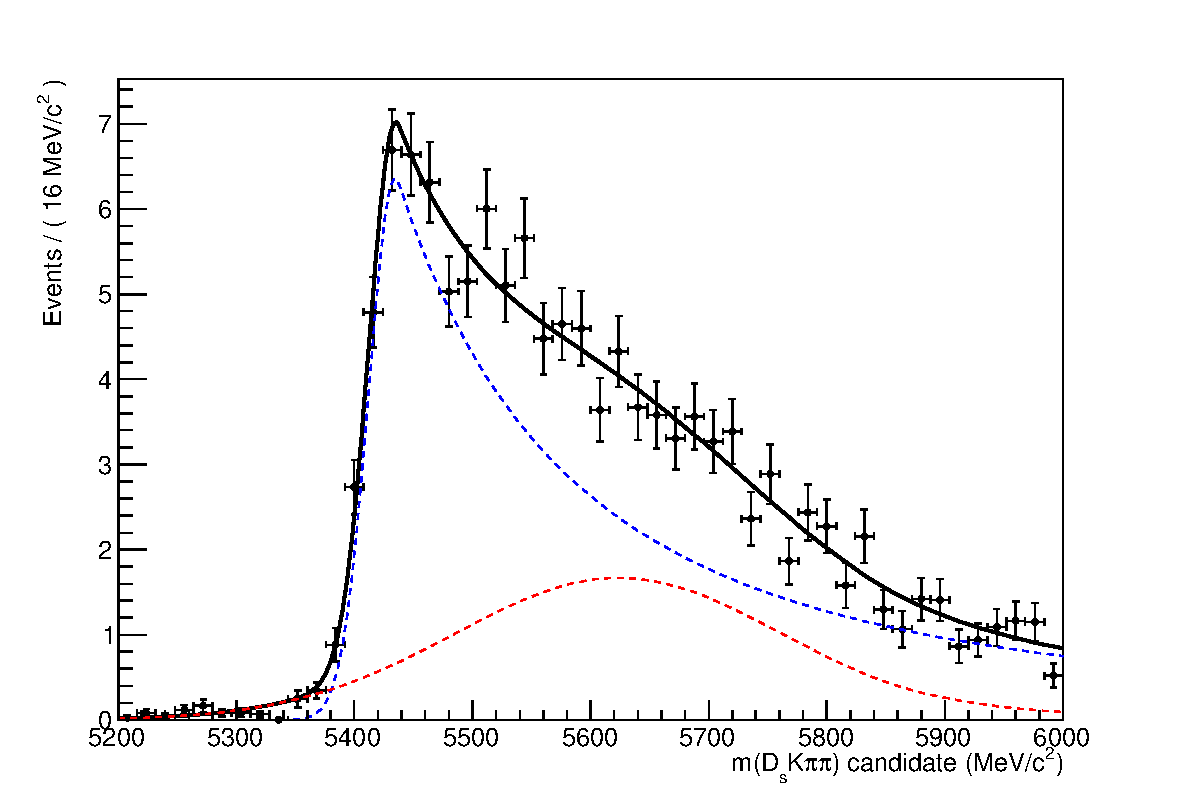
\includegraphics[height=6.cm,width=0.45\textwidth]{figs/Bs2Dspipipi_as_DsKpipi.pdf}
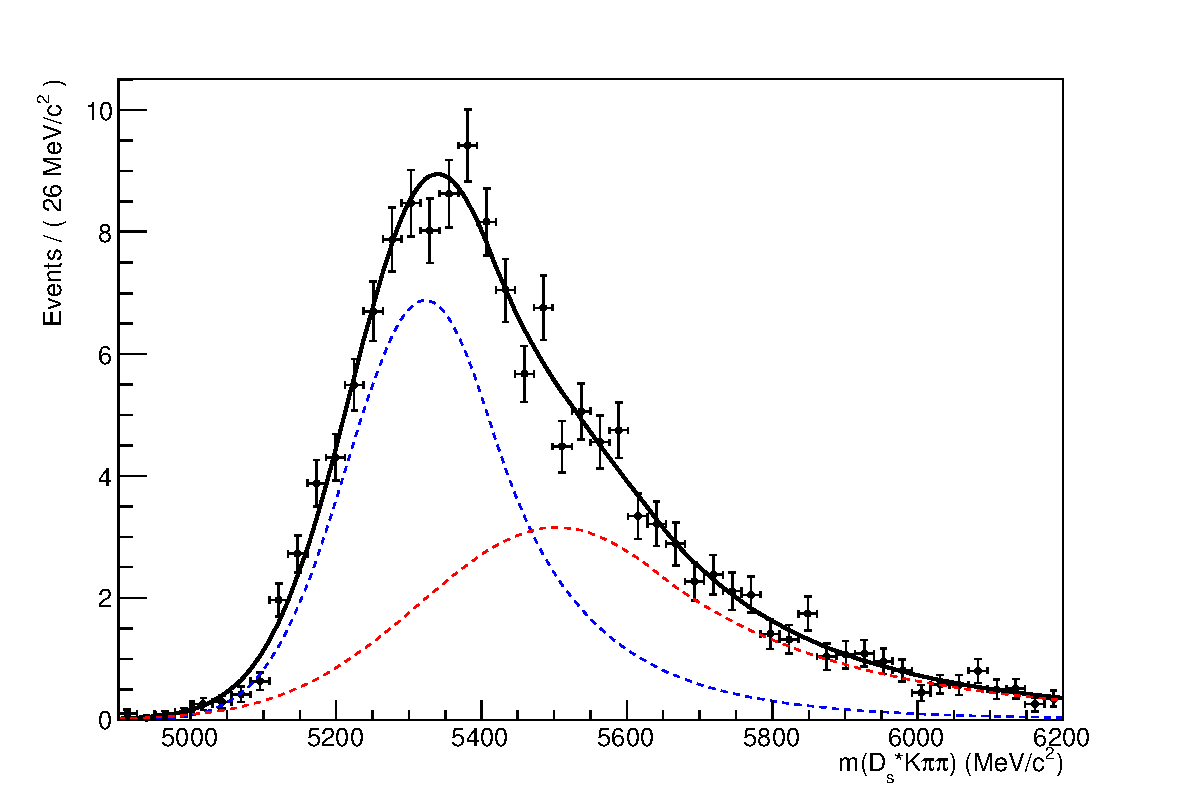
\includegraphics[height=6.cm,width=0.45\textwidth]{figs/Bs2Dsstarpipipi_as_DsKpipi.pdf}
\caption{Invariant mass distribution of (left) simulated $\Bs\to\Ds\pion\pion\pion$ events, where one of the $\pion$'s is reconstructed as a $\kaon$ and the misID probability for each event is taken into account. 
The corresponding distribution for simulated $\Bs\to\Ds^{*}\pion\pion\pion$ events, where the $\gamma$/$\piz$ from the $\Ds^{*}$ is excluded from reconstruction, is shown on the right.
The solid, black curve on each plot corresponds to the fit consisting of two Crystal Ball functions.}
\label{fig: BsDspipipiMCmissID}
\end{figure}
 
The expected yield of misidentified $\Bs\to\Ds\pion\pion\pion$ candidates in the $m(\Ds\kaon\pion\pion)$ spectrum is computed by multiplying the fake probability of $\propto3.2\%$, which is derived from PIDCalib, by the yield of $\Bs\to\Ds\pion\pion\pion$ signal candidates, determined in the nominal mass fit of our normalization channel.  \newline
In the same way as mentioned above, we can determine the rate of misidentified, partially reconstructed $\Bs\to\Ds^{*}\pion\pion\pion$ decays in our sample of $\Bs\to\Ds\kaon\pion\pion$ decays using PIDCalib and a MC sample of $\Bs\to\Ds^{*}\pion\pion\pion$ events. The invariant mass distribution we obtain when we exclude the $\gamma$/$\piz$, flip the the particle hypothesis $\pion\rightarrow\kaon$ and apply the event weights given by the fake rate, is shown in Fig. \ref{fig: BsDspipipiMCmissID} (right). The fit of two Crystal Ball functions to this distribution is overlaid. 
The yield of this contribution is determined from the yield of $\Bs\to\Ds^{*}\pion\pion\pion$ candidates in the nominal mass fit of our normalization channel, multiplied by the misID probability of $\propto 3.6\%$.


